\documentclass{beamer}

\mode<presentation> {
	\usetheme{Boadilla}
	%\usetheme{CambridgeUS}
}
\usefonttheme[onlymath]{serif}
\usepackage{graphicx}
\usepackage{booktabs} % Allows the use of \toprule, \midrule and \bottomrule in tables
\usepackage{amssymb,mathrsfs,amsmath}
\usepackage{amsfonts}
\usepackage{enumerate}
\usepackage{color}
%-------------------------------------------------------------------------

\title[Annu. Rev. Econ, 2009]{Sufficient Statistics for Welfare Analysis \\ {\small A Bridge Between Structural and Reduced-form Methods}}
\author{Chetty Raj} 
\institute[]{Presenter: Qinzhu Sun}

\date{\today}
\logo{
\includegraphics[scale=0.2]{maingate2}}
\begin{document}

\begin{frame}
	\titlepage
\end{frame}

\begin{frame}{Overview}
	\tableofcontents
\end{frame}
%-------------------------------------------------------------------------
%-------------------------------------------------------------------------
\section{Introduction}
\begin{frame}[shrink]
	\transfade %fade in and fade out
	\tableofcontents[sectionstyle=show/shaded,subsectionstyle=show/shaded/hide]
	\addtocounter{framenumber}{-1}
\end{frame}
%------------------------------------------------
\begin{frame}{Motivation}
	Two competing paradigms for policy evaluation and welfare analysis:
	\begin{block}{Structural approach}
		\begin{itemize}
			\item \textbf{Idea:} specify complete models of economic behavior and estimates or calibrates the primitives of models; simulate the effects of changes in policies and the economic environment on behavior and welfare.
			\item \textbf{Critique:} hard to identify all primitive parameters in an empirically compelling manner because of selection effects, simultaneity bias, and omitted variables.
		\end{itemize}
	\end{block}
	\begin{block}{Reduced-form approach}
		\begin{itemize}
			\item \textbf{Idea:} identify causal effects mainly using research	designs that exploit quasi-experimental variation.
			\item \textbf{Critique:} the estimates are not policy-invariant/ deep parameters of economic models and therefore have limited relevance for policy and welfare analysis.
		\end{itemize}
	\end{block}
\end{frame}
%------------------------------------------------
\begin{frame}
	\begin{figure}[h]
		\centering
		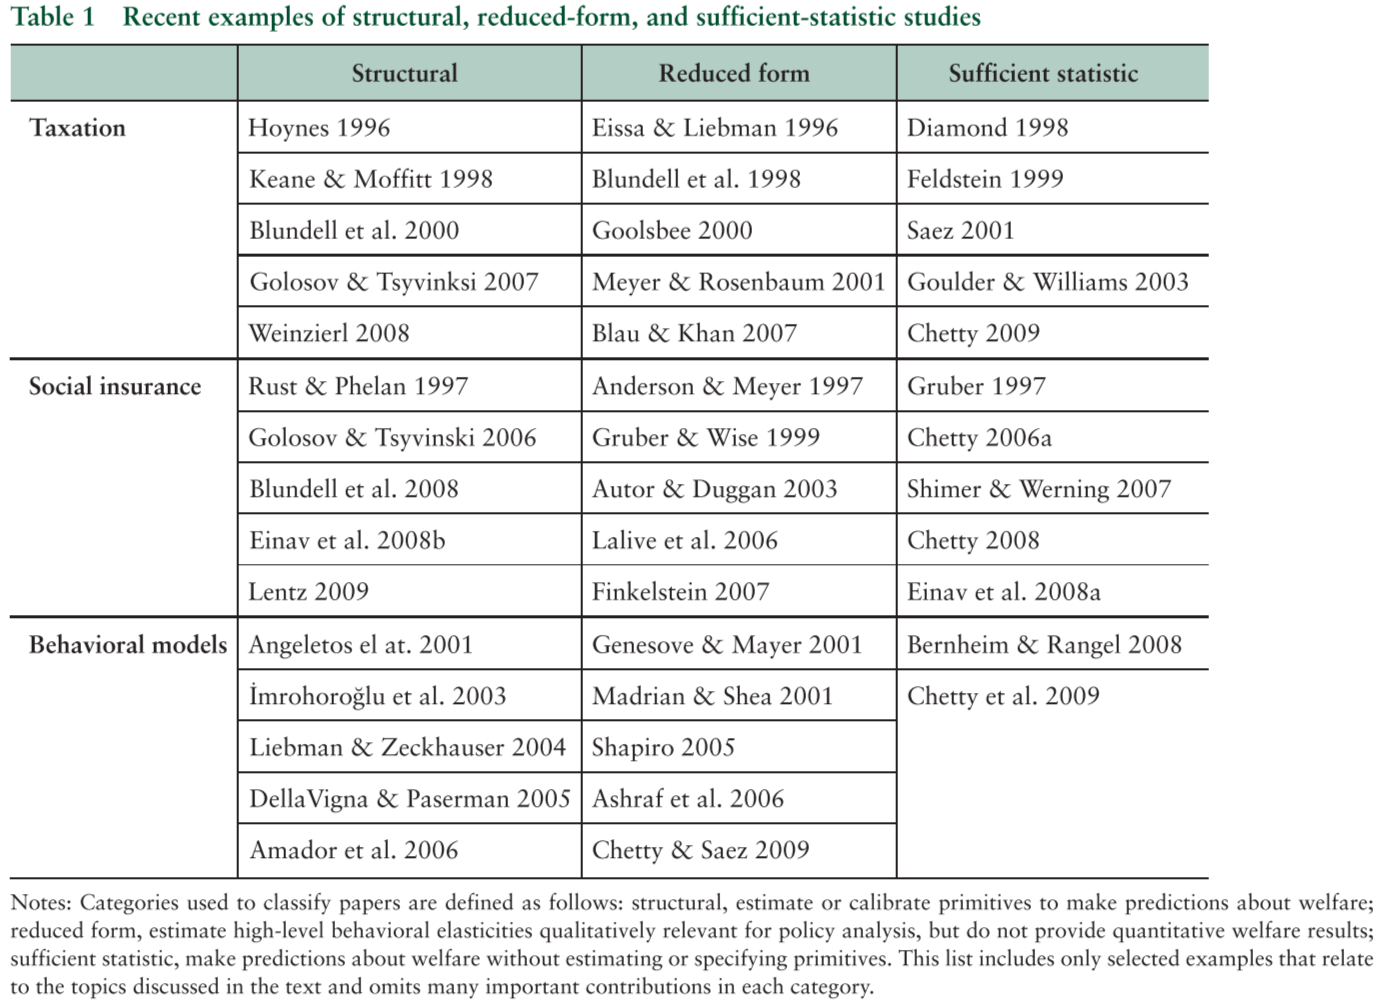
\includegraphics[scale=0.65]{table1.png}
	\end{figure}
\end{frame}
%------------------------------------------------
\begin{frame}{Sufficient Statistics}
	\textbf{A middle ground between the two methods:} develop sufficient-statistic formulas that combine 1) the advantages of reduced-form empirics, \textit{transparent and credible identification}, with 2) an important advantage of structural models, \textit{the ability to make precise statements about welfare}.
	\medskip
	\begin{itemize}
		\item Central concept: identify “sufficient statistics” for welfare analysis that can be estimated using reduced-form methods, rather than deep primitives.
		\item Even though there are multiple combinations of primitives that are consistent with the inputs to the formulas, all such combinations have the same welfare implications.
	\end{itemize}
\end{frame}
%------------------------------------------------
\begin{frame}{Sufficient Statistics}
	\begin{figure}[h]
		\centering
		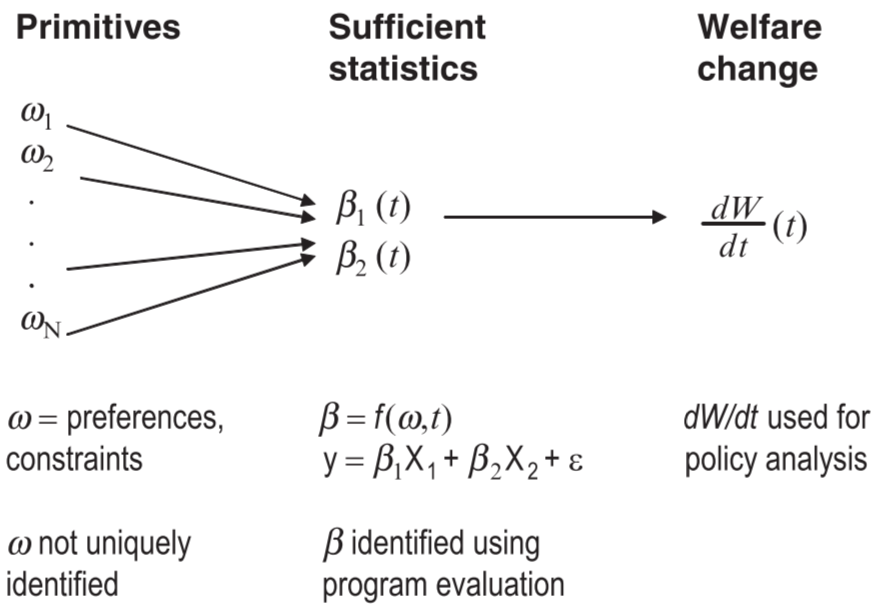
\includegraphics[scale=0.7]{figure1.png}
	\end{figure}
\end{frame}
%------------------------------------------------
\begin{frame}{Framework}
	\begin{enumerate}
		\item A general framework for the derivation of sufficient-statistic formulas for welfare analysis
		\begin{itemize}
			\item This framework shows how envelope conditions from optimization can be used to reduce the set of parameters that need to be identified.
		\end{itemize}
		\item A review of several recent papers on tax policy, social insurance, and behavioral public finance.
	\end{enumerate}
	\medskip
	\begin{block}{Marschak's maxim}
		\textit{"...for many decisions (policy problems), only combinations of explicit economic parameters are required -- no single economic parameter need be identified."}
		\hfill \textit{-- Heckman \& Vytlacil (2007)}
	\end{block}
\end{frame}
%------------------------------------------------
\begin{frame}{Pros \& Cons of Sufficient-statistic Approach}
	\textbf{Pros:}
	\begin{itemize}
		\item need to identify fewer parameters
		\item weaker modeling assumptions
		\item applicable when positive model that generates observed behavior is unknown (behavioral econ)
	\end{itemize}
	\textbf{Cons:}
	\begin{itemize}
		\item new formula must be derived for each question
		\item easily misapplied because no model evaluation required
		\item out-of-sample predictions may be less reliable
	\end{itemize}
	\medskip
	$\Rightarrow$ Sufficient statistic methods provide useful \textbf{complement} to (rather than a substitute for) structural methods.
\end{frame}
%-------------------------------------------------------------------------
%-------------------------------------------------------------------------
\section{A Precedent: Measuring Deadweight Loss}
\begin{frame}[shrink]
	\transfade %fade in and fade out
	\tableofcontents[sectionstyle=show/shaded,subsectionstyle=show/shaded/hide]
	\addtocounter{framenumber}{-1}
\end{frame}
%------------------------------------------------
\begin{frame}{Setup}
	Consider a static general equilibrium model:
	\begin{itemize}
		\item An individual is endowed with $Z$ units of numeraire $y$ ;
		\item Firms convert $y$ into $J$ other consumption goods $x=(x_1,...,x_J)$ ;
		\item $c(x)=\sum_{j=1}^Jc_j(x_j)$ is total cost of producing $x$ ;
		\item Perfectly competitive production ;
		\item The government levies a unit tax $t$ on good 1 ;
		\item $p=(p_1,...,p_J)$ is the pretax prices.
	\end{itemize}
\end{frame}
%------------------------------------------------
\begin{frame}{Setup}
	\textbf{Consumer side:}
	\begin{equation}
		\begin{aligned}
			\max_{x,y} u(x_1,...,x_J)+y \\
			\mbox{s.t. } p\cdot x + tx_1 + y = Z
		\end{aligned}
	\end{equation}

	\textbf{Producer side:}
	\begin{equation}
		\max_x p\cdot x - c(x)
	\end{equation}

	\textbf{Market-clearing condition:}
	\begin{equation}
		x^D(p) = x^S(p)\quad \Rightarrow \quad p^* = p(t)
	\end{equation}
\end{frame}
%------------------------------------------------
\begin{frame}{Measuring the Efficiency Cost}
	\textbf{How to measure the efficiency(deadweight) cost of tax $t$ ?}
	\medskip

	With quasi-linear utility, the consumer always allocates the lump-sum rebate to consumption of the numeraire y. Social welfare can then be written as the sum of the consumer’s utility, producer profits, and tax revenue:
	\begin{equation}\label{welfare}
		\begin{aligned}
			W(t) &= \{\max_x u(x) + Z - tx_1 - p(t)\cdot x \} + \{\max_x p(t)\cdot x - c(x)\} + tx_1 \\
			&= \{\max_x u(x) + Z - tx_1 - c(x)\} + tx_1.
		\end{aligned}
	\end{equation}

	$\Rightarrow$ The efficiency cost is actually $dW/dt$.
\end{frame}
%------------------------------------------------
\begin{frame}{Measuring the Efficiency Cost}
	There are two ways to estimate the effect of tax on social welfare $\frac{dW}{dt}$:
	\begin{block}{First approach}
		Estimate (or calibrate) a $J$ good demand and supply system to recover the utility function $u(x)$ and cost function $c(x)$. Once $u$ and $c$ are known, directly compute $W(t)$. Preferences can be recovered using the parametric demand systems; alternatively, one can fit a demand system to the data and then integrate to obtain the expenditure function.
		\begin{itemize}
			\item Challenge: simultaneity. Identifying the slope of the supply and demand curves requires $2J$ instruments.
		\end{itemize}
	\end{block}
\end{frame}
%------------------------------------------------
\begin{frame}{Measuring the Efficiency Cost}
	\begin{block}{Second approach $\star$}
		Harberger (1964) proposed an alternative, simpler solution to the problem. Differentiating Equation (\ref{welfare}) using the \textcolor{red}{envelope theorem}.
		\begin{equation}\label{welfare change}
			\frac{dW(t)}{dt} = -x_1 + x_1 + t\frac{dx_1}{dt} = t\frac{dx_1(t)}{dt}
		\end{equation}

		$\Rightarrow$ $\frac{dx_1}{dt}$ is a \textcolor{red}{sufficient stat} for analyzing the efficiency costs of tax changes.
		\begin{itemize}
			\item \textcolor{red}{Key point:} the full system of supply and demand curves does not have to be identified to calculate $\Delta W$.
			\item The loss in social surplus is determined purely by the difference between the agent’s willingness to pay for good $x_1$ and the cost of producing good $x_1$.
			\item The \textcolor{red}{simplicity} of Harberger’s approach stems from estimating $\frac{dx_1}{dt}$ directly rather than estimating its various components, which is effectively what the structural approach requires.
		\end{itemize}
	\end{block}
\end{frame}
%------------------------------------------------
\begin{frame}{Measuring the Efficiency Cost}
	\begin{figure}[h]
		\centering
		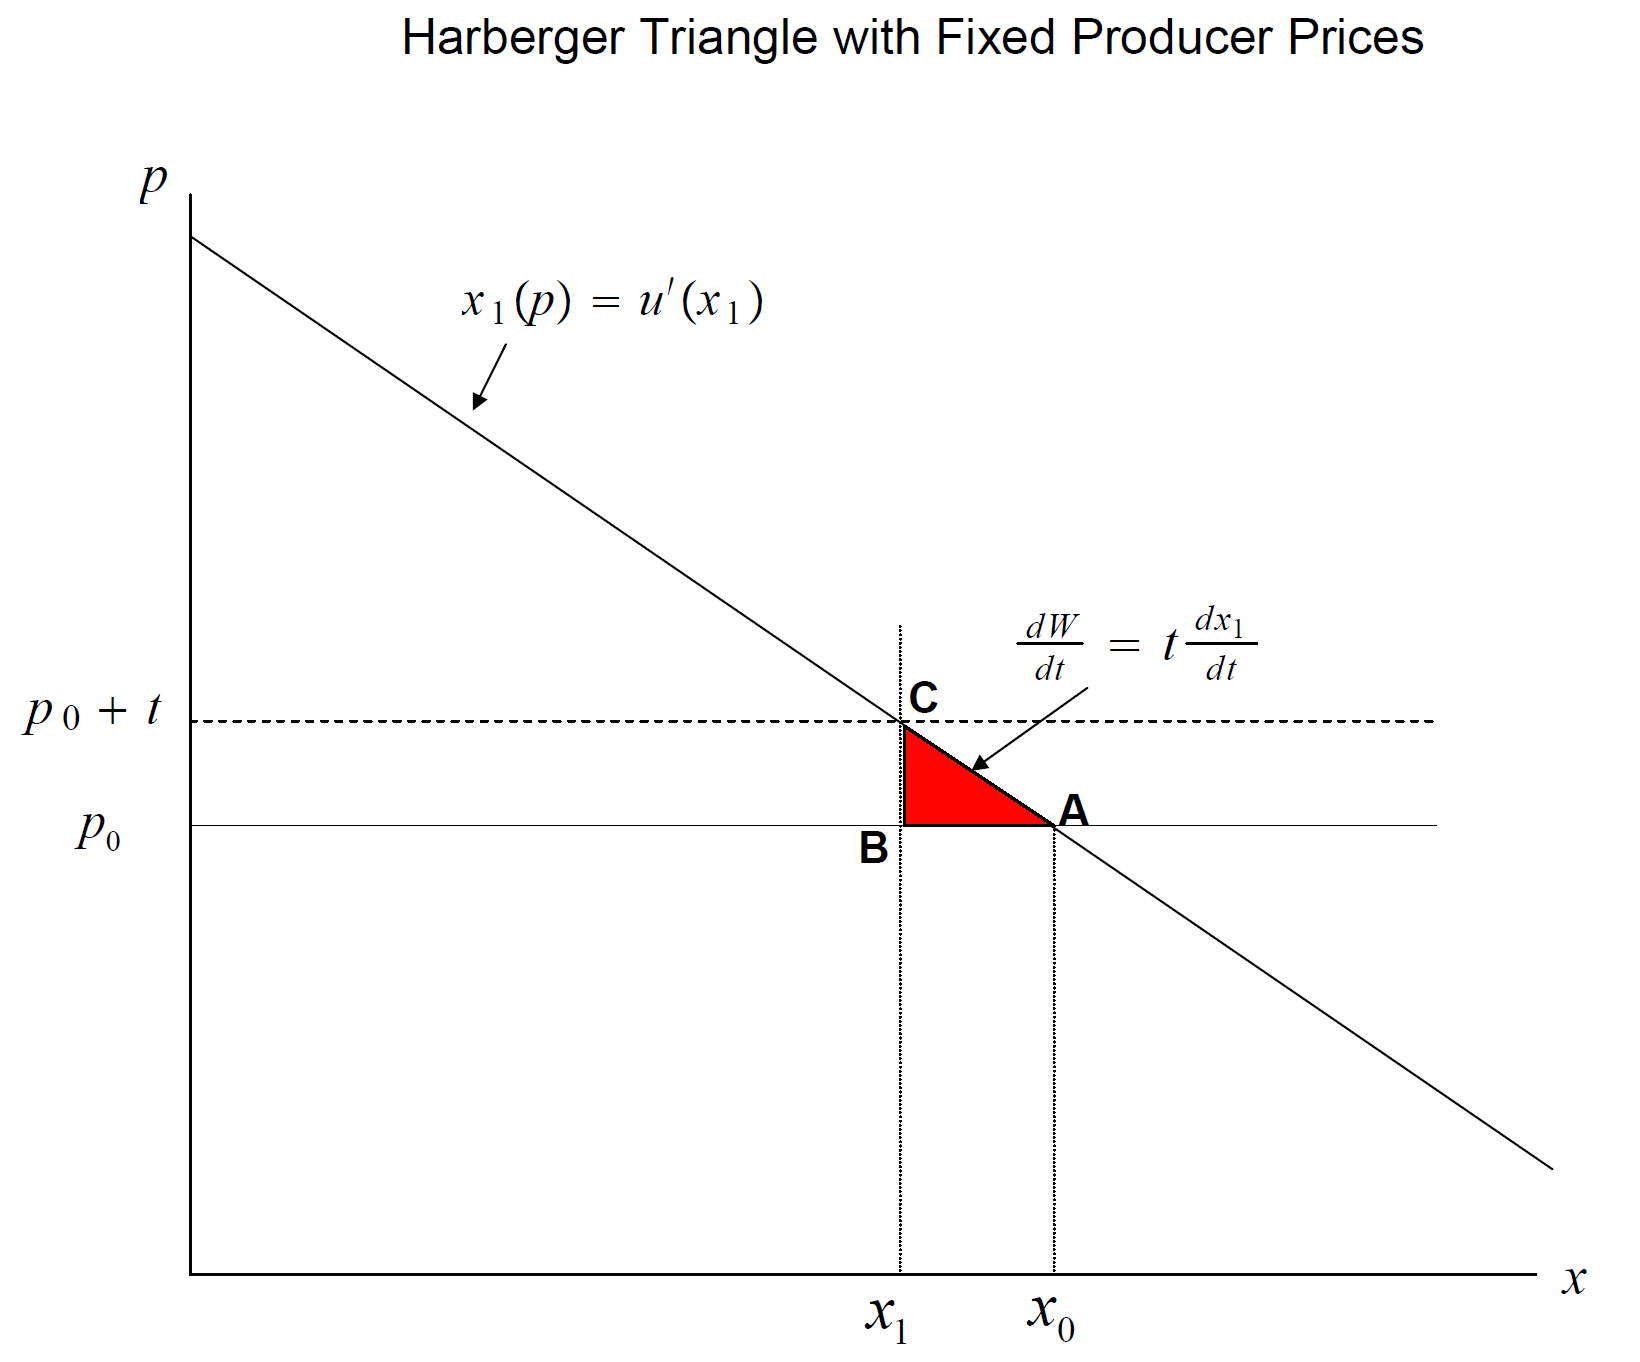
\includegraphics[scale=0.44]{harberger_tri.png}
	\end{figure}	
\end{frame}
%------------------------------------------------
\begin{frame}{A Brief Summary}
	\textbf{Limitations of Harberger's approach:}
	\begin{itemize}
		\item It does not permit pre-existing distortions in the other markets; otherwise the spillover effects would have first-order effects on welfare.
		\item it cannot be used directly to evaluate counterfactual policy changes, such as the imposition of a large new tax on good $x_1$.
	\end{itemize}
	\medskip

	\textbf{Benefits of Harberger’s approach:}
	\begin{itemize}
		\item It permits heterogeneity across individuals and discrete choice. $\Rightarrow$ Two extensive examples since next page...
	\end{itemize}
\end{frame}
%------------------------------------------------
\begin{frame}{Extension 1: Heterogeneity}
	Individual $i$ is endowed with $Z_i$ units of the numeraire and has utility
	\begin{equation}
		u^i(x^i) + y.
	\end{equation}
	\begin{equation}
		\Rightarrow W(t) = \left\{\sum_{i=1}^N\max_{x^i}\left[u^i(x^i)+Z^i-tx_1^i\right]-c(x) \right\} + t\sum_{i=1}^Nx_1^i
	\end{equation}
	\begin{equation}\label{ex1}
		\Rightarrow \frac{dW(t)}{dt} = -\sum_{i=1}^N x_1^i + \sum_{i=1}^N x_1^i + t\frac{d\sum_{i=1}^Nx_1^i}{dt} = t\frac{dx_1(t)}{dt}.
	\end{equation}

	So $\frac{dx_1}{dt}$ is a sufficient statistic for the marginal excess tax burden.
	\begin{itemize}
		\item There is no need to characterize the underlying heterogeneity in the population to implement Equation (\ref{ex1});
		\item Even though each individual diverges in demand elasticity, what matters for government revenue and aggregate welfare is the total change in behavior induced by the tax.
	\end{itemize}
\end{frame}
%------------------------------------------------
\begin{frame}{Extension 2: Discrete Choice}
	\textbf{Setup:}
	\begin{itemize}
		\item Individuals choose one of the $J$ products $\{1,...,J\}$ ;
		\item Each product is characterized by a vector of K observable attributes $x_j=(x_{1j},...,x_{Kj})$ and an unobservable attribute $\zeta$ ;
	\end{itemize}
	If agent $i$ chooses product $j$, his utility is
	\begin{equation}
		\begin{aligned}
			u_{ij} &= v_{ij} + \varepsilon_{ij}, \\
			\mbox{with } v_{ij} &= Z^i - p_j + \zeta_j + \phi^i(x_j).
		\end{aligned}
	\end{equation}

	\textbf{Denotation:}
	\begin{itemize}
		\item $P_{ij}$ : the probability that individual $i$ chooses option $j$ ;
		\item $P_j=\sum_i P_{ij}$ : total (expected) demand for product $j$ ;
		\item $P=(P_1,...,P_J)$ : the vector of aggregate product demands;
		\item Product $j$ is produced using $c_j(P_j)$ units of the numeraire $y$, and $c(P)=\sum_j c_j(P_j)$.
	\end{itemize}
\end{frame}
%------------------------------------------------
\begin{frame}{Extension 2: Discrete Choice}{Binary Choice Case}
	Suppose individuals make binary decisions about whether to buy $x_1$.
	\begin{itemize}
		\item If he doesn't buy $x_1$ and spends wealth on y, obtain utility $u_i = Z^i$ ;
		\item If he buys $x_1$, his utility is $u_i=Z^i-p_1+\zeta_1+\phi^i(x_1)+\varepsilon_{i1}$ .
	\end{itemize}
	\textbf{Denotation:}
	\begin{itemize}
		\item $V_i=\zeta_i+\phi^i(x_1)+\varepsilon_{i1}$ : individual $i$'s gross valuation of $x_1$ ;
		\item $F(V^i)$ : the smooth distribution of valuations in the economy;
		\item $EZ$ : the average level of wealth in the economy;
		\item $\bar{V}$ : the cutoff of $V_i$ to buy $x_1$.
	\end{itemize}
	\begin{equation}
		W(t) = \left\{EZ + \max_{\bar{V}}\int_{\bar{V}}^\infty\left[V^i-(p_1+t)\right]dF(V^i)\right\} + t\int_{\bar{V}}^\infty dF(V^i)
	\end{equation}
	\begin{equation}
		\frac{dW}{dt} = -\left[1-F(\bar{V})\right] + \left[1-F(\bar{V})\right] + t\frac{d\int_{\bar{V}}^\infty dF(V^i)}{dt} = t\frac{dx_1}{dt}
	\end{equation}
\end{frame}
%------------------------------------------------
\begin{frame}{Extension 2: Discrete Choice}{Multinomial Choice Case}
	Assume that $\varepsilon_{ij}$ has a type I extreme value distribution. $\Rightarrow$ The probability that a utility-maximizing individual $i$ chooses product $j$ is
	\begin{equation}
		P_{ij} = \frac{\exp(v_{ij})}{\sum_j \exp(v_{ij})}
	\end{equation}
	and that agent $i$'s expected utility from price vector $p=(p_1,...,p_J)$ is
	\begin{equation}
		S_i(p_1,...,p_J) = E\max(u_{i1},...,u_{iJ}) = \log \left(\sum_j\exp(v_{ij})\right).
	\end{equation}

	Aggregating over $i=1,...,N$ consumers, (expected) consumer surplus is
	\begin{equation}
		S = \sum_i\log\left(\sum_j\exp(v_{ij}) \right).
	\end{equation}
\end{frame}
%------------------------------------------------
\begin{frame}{Extension 2: Discrete Choice}{Multinomial Choice Case}
	Add producer profits to obtain social welfare:
	\begin{equation}
		W = \sum_i\log\left(\sum_j\exp(v_{ij})\right) + p\cdot P-c(P)
	\end{equation}

	Sufficient-statistic approaches offer a means of policy analysis that does not require identifying $\phi_i$ and $\zeta_j$. Suppose the government levies a tax $t$ on good 1, raising its price to $p_1+t$. The proceeds are returned to agents through a lump-sum transfer $T$ so that $y_i$ becomes $y_i+T$.
	\begin{equation}
		\begin{aligned}
			\Rightarrow \frac{dW(t)}{dt} &= \sum_i\left[-\frac{\exp(v_{i1})}{\sum_j \exp(v_{ij})} - \sum_j\frac{dp_j}{dt}\frac{\exp(v_{ij})}{\sum_j \exp(v_{ij})} \right] \\
			&+ \sum_j\frac{dp_j}{dt}P_j + P_1 + t\frac{dP_1}{dt} = t\frac{dP_1(t)}{dt}.
		\end{aligned}
	\end{equation}
\end{frame}
%------------------------------------------------
\begin{frame}{Extension 2: Discrete Choice}{Multinomial Choice Case}
	Now suppose that an ad-valorem tax $t$ is levied on all the products except the numeraire good, raising the price of product $j$ to $(1+\tau)p_j$. Similarly,
	\begin{equation}
		\frac{dW(\tau)}{d\tau} = \tau\sum_j p_j\frac{dP_j(\tau)}{d\tau} = \tau\frac{dE_P(\tau)}{d\tau},
	\end{equation}
	where $E_p=\sum_j p_jP_j$ denotes total pretax expenditure for the taxed good.
	\begin{itemize}
		\item Finding: The efficiency cost of a tax on all products depends on the aggregate expenditure elasticity for the taxed market; it does not require estimation of the substitution patterns within that market.
	\end{itemize}
	\medskip

	$\Rightarrow$ Hence, many policy questions of interest can be answered simply by estimating reduced-form aggregate demand responses even in discrete choice models.
\end{frame}
%-------------------------------------------------------------------------
%-------------------------------------------------------------------------
\section{General Framework}
\begin{frame}[shrink]
	\transfade %fade in and fade out
	\tableofcontents[sectionstyle=show/shaded,subsectionstyle=show/shaded/hide]
	\addtocounter{framenumber}{-1}
\end{frame}
%------------------------------------------------
\begin{frame}[label=ex_harberger]{Specify the Model Structure}
	\textbf{Consumer decision:}
	\begin{equation}
		\max U(x)\mbox{ s.t. } G_1(x,t,T) = 0,...,G_M(x,t,T) = 0.
	\end{equation}

	\begin{itemize}
		\item A unit tax $t$ is levied on choice $x_1$ and the transfer $T(t)$ is paid in units of $x_J$ ;
		\item $\{G_1(x,t,T),...,G_M(x,t,T)\}$ denote the $M<J$ constraints.
	\end{itemize}
	\begin{equation}
		\Rightarrow W(t) = \max_x U(x) + \sum_{m=1}^M\lambda_mG_m(x,t,T).
	\end{equation}
	
	\begin{block}{An example of single-agent Harberger model \hyperlink{ex_hgb_back}{\beamergotobutton{Back}}}
		\begin{equation}\nonumber
			\begin{aligned}
				U(x) &= u(x_1,...,x_{J-1}) + x_J \\
				G_1(x,t,T) &= T + Z - tx_1 - c(x_1,...,x_{J-1}) - x_J
			\end{aligned}
		\end{equation}
	\end{block}
\end{frame}
%------------------------------------------------
\begin{frame}{Express $dW/dt$ in Terms of Multipliers}
	Using the envelope conditions,
	\begin{equation}\label{foc_eq14}
		\frac{dW}{dt} = \sum_{m=1}^M\lambda_m\left\{\frac{\partial G_m}{\partial T}\frac{dT}{dt}+\frac{\partial G_m}{\partial t}\right\}.
	\end{equation}

	\begin{itemize}
		\item $\frac{dT}{dt}$ is known through the govt's budget constraint;
		\item $\frac{\partial G_m}{\partial T}$ and $\frac{\partial G_m}{\partial t}$ can be calculated mechanically.
	\end{itemize}
	\medskip

	$\Rightarrow$ The critical unknowns are the $\lambda_m$ multipliers.
\end{frame}
%------------------------------------------------
\begin{frame}{Substitute Multipliers by Marginal Utilities}
	The $\lambda_m$ multipliers are recovered by exploiting restrictions from the agent’s first-order conditions:
	\begin{equation}\nonumber
		u'(x_j) = -\sum_{m=1}^M\lambda_m\frac{\partial G_m}{\partial x_j}
	\end{equation}

	Inverting this system of equations generates a map from the multipliers into the marginal utilities. To simplify this mapping, impose the following assumption:
	\begin{block}{Assumption 1 (Interchangability Condition)}
		\begin{equation}\label{assumption1}\nonumber
			\begin{aligned}
				\frac{\partial G_m}{\partial t} &= k_t(x,t,T)\frac{\partial G_m}{\partial x_1} &\forall m=1,...,M, \\
				\frac{\partial G_m}{\partial T} &= -k_T(x,t,T)\frac{\partial G_m}{\partial x_J} &\forall m=1,...,M
			\end{aligned}
		\end{equation}
	\end{block}
\end{frame}
%------------------------------------------------
\begin{frame}{Substitute Multipliers by Marginal Utilities}
	Substitute Assumption 1 into equation (\ref{foc_eq14}) to obtain
	\begin{equation}
		\begin{aligned}
			\frac{dW}{dt} &= \sum_{m=1}^M\lambda_m\left\{-k_T\frac{\partial G_m}{\partial x_J}\frac{dT}{dt} + k_t\frac{\partial G_m}{\partial x_1}\right\} \\
			&= -k_T\frac{dT}{dt}\sum_{m=1}^M\lambda_m\frac{\partial G_m}{\partial x_J} + k_t\sum_{m=1}^M\lambda_m\frac{\partial G_m}{\partial x_1} \\
			&= k_T\frac{dT}{dt}u'(x_J(t)) - k_tu'(x_1(t)).
		\end{aligned}
	\end{equation}

	\begin{block}{Intuition}
		Increasing the tax $t$ is equivalent to reducing consumption of $x_1$ by $k_t$ units, which reduces the agent’s utility by $k_tu'(x_1(t))$. Since $k_T$, $k_t$, and $\frac{dT}{dt}$ are known based on model specification, this expression distills local welfare analysis to recovering a pair of marginal utilities.
	\end{block}
\end{frame}
%------------------------------------------------
\begin{frame}[label=ex_hgb_back]{Recover Marginal Utilities from Observed Choices}
	The final step in obtaining an empirically implementable expression for $\frac{dW}{dt}$ is to back out the two marginal utilities.
	\begin{itemize}
		\item Sufficient-statistic studies recover the marginal utilities from choice data using the model structure specified in step 1. There is no canned procedure for this step.
		\item The usual trick is that the marginal utilities are elements in first-order conditions for various choices. As a result, they can be backed out from the comparative statics of behavior.
	\end{itemize}
	\begin{block}{Example: Single-agent Harberger Model \hyperlink{ex_harberger}{\beamergotobutton{Example}}}
		The assumption of no income effects implies $u'(x_J)=1$. The first-order condition for $x_1$ leads to $u'(x_1)=p_1+t$.
		\begin{equation}\nonumber
			\Rightarrow \frac{dW(t)}{dt} = 1\cdot \left(x_1+t\frac{dx_1}{dt}\right)-\frac{x_1}{p_1+t}\cdot (p_1+t) = t\frac{dx_1(t)}{dt}.
		\end{equation}
	\end{block}
\end{frame}
%------------------------------------------------
\begin{frame}{Empirical Implementation}
	Suppose the sufficient-statistic formula has the following form:
	\begin{equation}\label{eq16}
		\frac{dW}{dt}(t) = f\left(\frac{\partial x_1}{\partial t},\frac{\partial x_1}{\partial Z},t \right).
	\end{equation}
	\begin{block}{Note 1}
		The relevant derivatives may require holding different variables fixed depending upon the application.
		\begin{itemize}
			\item E.g. the Harberger formula in Equation (\ref{welfare change}) measures $\frac{dx_1}{dt}$, which incorporates general equilibrium effects \& price changes in all markets.
			\item In contrast, many reduced-form empirical studies explicitly	identifies $\frac{\partial x_1}{\partial t}$, holding prices in other markets constant. Such studies do not recover the sufficient stat of interest for Harberger policy questions.
		\end{itemize}
		$\Rightarrow$ The \textcolor{red}{general lesson} is that the experiment used to identify the relevant elasticities must be matched to the policy question being asked.
	\end{block}
\end{frame}
%------------------------------------------------
\begin{frame}{Empirical Implementation}
	\begin{block}{Note 2}
		\begin{itemize}
			\item The ideal way to implement Equation (\ref{eq16}) to assess the efficiency costs of a discrete policy change is to estimate the inputs as \textcolor{red}{nonparametric} functions of the policy instrument $t$.
			\item With estimates of $\frac{\partial x_1}{\partial t}(t)$ and $\frac{\partial x_1}{\partial Z}(t)$, one can integrate Equation (\ref{eq16}) between any two tax rates $t_1$ and $t_2$ to evaluate $\Delta W$.
		\end{itemize}
	\end{block}
	\medskip

	In most applications, there is insufficient power to nonparametrically estimate $x_1(t)$. Instead, typical reduced-form studies estimate LATE, such as $\frac{\Delta x_1}{\Delta t}=\frac{x_1(t_2)-x_1(t_1)}{t_2-t_1}$.
\end{frame}
%------------------------------------------------
\begin{frame}{Empirical Implementation}
	To see this, consider the Harberger model $\frac{dW}{dt}(t)=t\frac{dx_1}{dt}(t)$. A researcher who has estimated $\frac{\Delta x_1}{\Delta t}$ has two options.
	\medskip

	\textbf{Option 1:} \textcolor{red}{bound} the average welfare gain over the observed range.
	\begin{equation}
		\begin{aligned}
			& W(t_2) - W(t_1) = \int_{t_1}^{t_2}\frac{dW}{dt}dt=\int_{t_1}^{t_2}t\frac{dx_1}{dt}(t)dt \\
			& \Rightarrow t_1\frac{\Delta x_1}{\Delta t}>\overline{dW/dt}>t_2\frac{\Delta x_1}{\Delta t}
		\end{aligned}
	\end{equation}

	\textbf{Option 2:} \textcolor{red}{approximate} to $x_1(t)$ to calculate $\overline{dW/dt}$. E.g.
	\begin{equation}
		\overline{dW/dt}\simeq \frac{t_1+t_2}{2}\frac{\Delta x_1}{\Delta t}
	\end{equation}
\end{frame}
%------------------------------------------------
\begin{frame}{Model Evaluation}
	Although sufficient-statistic formulas do not require full specification of the model, they do require some modeling assumptions. It is important to assess the \textcolor{red}{validity of these assumptions} to ensure the accuracy of results.
	\medskip

	The model can be evaluated in two ways.
	\begin{enumerate}
		\item One can test qualitative predictions that would falsify the assumptions that are central for deriving the sufficient-statistic formula.
		\item One should identify at least one vector of structural parameters $\omega$ that is consistent with the sufficient statistics estimated in step 5. If the empirical estimates of the sufficient statistics are internally consistent with the model, at least one $\omega$ must fit the estimated
		statistics.
	\end{enumerate}
\end{frame}
%-------------------------------------------------------------------------
%-------------------------------------------------------------------------
\section{Application 1: Income Taxation}
\begin{frame}[shrink]
	\transfade %fade in and fade out
	\tableofcontents[sectionstyle=show/shaded,subsectionstyle=show/shaded/hide]
	\addtocounter{framenumber}{-1}
\end{frame}
%------------------------------------------------
\begin{frame}{Income Taxation}{Feldstein (1999)}
	\textbf{Setup:}
	\begin{itemize}
		\item An ind makes $J$ labor-supply choices $(x_1,...,x_J)$ that generate income;
		\item $w_j$ denote the wage paid for choice $j$; $\psi_j(x_j)$ denote the disutility of labor supply through margin $x_j$ ;
		\item The agent shelters $e$ of earnings from the tax authority by paying $g(e)$;
		\item Total taxable income is $TI=\sum_{j=1}^Jw_jx_j-e$ ;
		\item Consumption is then $c = (1-t)TI+e$.
	\end{itemize}
	\begin{equation}
		u(c,x,e) = c-g(e)-\sum_{j=1}^J\psi_j(x_j)
	\end{equation}
	\begin{equation}
		\begin{aligned}
			T(t) &= t\cdot TI \\
			G_1(c,x,t) &= T + (1-t)TI + e - c
		\end{aligned}
	\end{equation}
\end{frame}
%------------------------------------------------
\begin{frame}{Income Taxation}{Feldstein (1999)}
	Social welfare is
	\begin{equation}\label{eq18}
		W(t) = \left\{(1-t)TI+e-g(e)-\sum_{j=1}^J\psi_j(x_j)\right\}+t\cdot TI.
	\end{equation}

	To calculate the marginal excess burden $\frac{dW}{dt}$, differentiate equation (\ref{eq18}):
	\begin{equation}\label{eq19}
		\begin{aligned}
			\frac{dW}{dt} &= TI + t\frac{dTI}{dt} - TI + (1-t)\frac{dTI}{dt}+\frac{de}{dt}(1-g'(e))-\sum_{j=1}^J\psi_j'(x_j)\frac{dx_j}{dt} \\
			&= \frac{dTI}{dt} + \frac{de}{dt}(1-g'(e)) - \sum_{j=1}^J\psi_j'(x_j)\frac{dx_j}{dt}.
		\end{aligned}
	\end{equation}
\end{frame}
%------------------------------------------------
\begin{frame}{Income Taxation}{Feldstein (1999)}
	To recover the marginal utilities (step 4), Feldstein exploited the F.O.C.
	\begin{equation}\label{eq20}
		\begin{aligned}
			g'(e) &= t \\
			\psi_j'(x_j) &= (1-t)w_j \Rightarrow \sum_{j=1}^J\psi_j'(x_j)\frac{dx_j}{dt} = \sum_{j=1}^J(1-t)w_j\frac{dx_j}{dt} = (1-t)\frac{d(TI+e)}{dt}
		\end{aligned}
	\end{equation}

	Plug equation (\ref{eq20}) into equation (\ref{eq19}), we obtain
	\begin{equation}\label{eq21}
		\frac{dW(t)}{dt} = t\frac{dTI(t)}{dt}.
	\end{equation}

	$\Rightarrow$ We simply need to measure how taxable income responds to changes in the tax rate to calculate the deadweight cost of income taxation.
\end{frame}
%------------------------------------------------
\begin{frame}{Income Taxation}{Feldstein (1999)}
	Chetty (2009) argued that the marginal social cost of tax avoidance may not
	be equal to the tax rate at the optimum, violating the F.O.C. (Equation (\ref{eq20})) that is critical to derive Equation (\ref{eq21}).
	\begin{enumerate}
		\item Some of the costs of evasion and avoidance constitute transfers rather than resource costs;
		\item There is considerable evidence that individuals overestimate the true penalties for evasion.
	\end{enumerate}
	Chetty relaxed the $g'(e)=t$ restriction and obtained the following generalization of Feldstein’s formula:
	\begin{equation}
		\frac{dW(t)}{dt} = t\left\{\mu(t)\frac{dTI(t)}{dt}+(1-\mu(t))\frac{dLI(t)}{dt}\right\},
	\end{equation}
	where $LI=\sum_{j=1}^Jw_jx_j$ represents total earned income and $\mu(t)=\frac{g'(e(t))}{t}$ measures the gap between social marginal costs of avoidance and tax rate.
\end{frame}
%------------------------------------------------
\begin{frame}{Income Taxation}{Saez (2001)}
	\textbf{Setup:}
	\begin{itemize}
		\item Individuals choose hours of work, $l$, and have heterogeneous wage rates $w$ distributed according to a distribution $F(w)$ ;
		\item Pretax earnings is denoted $z=wl$ ;
		\item The govt levies a linear tax $\tau$ on earnings above a threshold $\bar{z}$ ;
		\item $c(w,\tau)$, $l(w,\tau)$, $z(w,\tau)$ are the agent's optimal choices.
	\end{itemize}
	\medskip

	For a given $\bar{z}$, individuals maximize utility
	\begin{equation}
		\begin{aligned}
			u(c,l) &= c - \psi(l) \\
			\mbox{s.t. }G_1(c,l) &= (1-\tau)\max (wl-\bar{z},0) + \bar{z} - c = 0.
		\end{aligned}
	\end{equation}
\end{frame}
%------------------------------------------------
\begin{frame}{Income Taxation}{Saez (2001)}
	Let
	\begin{itemize}
		\item $z_m(\bar{z})=E[wl(w,\tau)|z(w,\tau)>\bar{z}]$ denote the mean level of earnings for individuals in the top bracket;
		\item $\bar{w}$ represent the wage threshold that corresponds to an earnings threshold of $\bar{z}$ when the tax rate is $\tau:\bar{w}l(\bar{w},\tau)=\bar{z}$.
	\end{itemize}
	$\Rightarrow$ The tax revenue generated by the top bracket tax is $R=\tau(z_m(\bar{z})-\bar{z})$.
	\medskip

	\textbf{Social planner’s objective:} maximize a weighted average of individual’s utilities, where the weights $\tilde{G}(u)$ are social-welfare weights that reflect the redistributive preferences of the planner.
	\begin{equation}
		W=\left\{\int_0^\infty \tilde{G}(u(c(w,\tau),wl(w,\tau)))dF(w)\right\} + \tau(z_m(\bar{z})-\bar{z})
	\end{equation}
\end{frame}
%------------------------------------------------
\begin{frame}{Income Taxation}{Saez (2001)}
	\begin{equation}
		\begin{aligned}\label{eq23}
			\Rightarrow \frac{dW}{d\tau}(\tau) &= -\int_{\bar{w}}^\infty\tilde{G}_u(u)(z(w,\tau)-\bar{z})dF(w) + \left[(z_m-\bar{z})+\tau\frac{dz_m}{d\tau}\right] \\
			&= -(z_m(\bar{z})-\bar{z})\bar{g} + \left[(z_m(\bar{z})-\bar{z})+\tau\frac{dz_m}{d\tau}\right],
		\end{aligned}
	\end{equation}
	where
	\begin{itemize}
		\item $\bar{g}=\int_{\bar{w}}^\infty \tilde{G}_u(u)(z-\bar{z})dF(w)/\int_{\bar{w}}^\infty (z-\bar{z})dF(w)$ denotes the mean marginal social-welfare weight placed by the planner on individuals in the top tax bracket;
		\item $\bar{g}$ measures the social value of giving \$1 more income to individuals in the top bracket relative to the value of public expenditure.
	\end{itemize}
	\medskip

	$\Rightarrow$ $\frac{dz_m}{d\tau}$, $z_m(\bar{z})$, $\bar{g}$ are together sufficient statistics for the welfare gain of increasing top income-tax rates.
\end{frame}
%------------------------------------------------
\begin{frame}{Income Taxation}{Saez (2001)}
	Saez observed that the upper tail of the earnings distribution is well described by a Pareto distribution in US.\footnote{A Pareto distribution with parameter $a$ has $\frac{z_m(\bar{z})}{\bar{z}}=\frac{a}{a-1}$ for all $\bar{z}$.} Hence, equation (\ref{eq23}) can be expressed as
	\begin{equation}
		\frac{dW}{dt} = \frac{1-\bar{g}}{a-1}\bar{z} + \tau\frac{dz_m}{d\tau}.
	\end{equation}

	The optimal top-bracket tax rate $\tau$ satisfies $\frac{dW}{d\tau}(\tau)=0$, implying
	\begin{equation}\label{eq24}
		\frac{\tau^*}{1-\tau^*} = \frac{1-\bar{g}}{a\varepsilon},
	\end{equation}
	where $\varepsilon=\frac{dz_m}{d(1-\tau)}\frac{1-\tau}{z_m}$ is the taxable income elasticity in the top bracket.
	\medskip

	$\Rightarrow$ Equation (\ref{eq24}) is an explicit formula for the optimal asymptotic top income-tax rate.
\end{frame}
%------------------------------------------------
\begin{frame}{Income Taxation}{Saez (2001)}
	Saez characterized the optimal tax rate in a nonlinear tax system.
	
	\textbf{Denotation:}
	\begin{itemize}
		\item $\varepsilon(z)=\frac{dz}{d(1-\tau)}\frac{1-\tau}{z}$ : the earnings elasticity at income level $z$ ;
		\item $h(z)$ : the density of the earnings distribution at $z$ ;
		\item $\tilde{G}(u(z))$ : the weight that the planner places on an individual;
		\item $g(Z)=\tilde{G}_u\cdot u_c(z)$ is the marginal social-welfare weight.
	\end{itemize}
	\medskip

	The government chooses the schedule $T(Z)$ that maximizes social welfare
	\begin{equation}\nonumber
		\begin{aligned}
			W(T(z)) &= \int_0^\infty\tilde{G}(u(c(w,T),wl(w,T)))dF(w) \\
			\mbox{s.t. }G_1(c,z,T) &= \int_0^\infty z(w,T)dF(w)-\int_0^\infty c(w,T)dF(w)-E=0 \mbox{ (RC)} \\
			G_2(c,z,T) &= (1-T'(z))w-\psi'(l(w))=0 \mbox{ (IC)}
		\end{aligned}
	\end{equation}
\end{frame}
%------------------------------------------------
\begin{frame}{Income Taxation}{Saez (2001)}
	Exploiting envelope conditions and perturbation arguments as above, the optimal tax schedule satisfies the following condition at all $z$:
	\begin{equation}
		\frac{T(z)}{1-T(z)} = \frac{1}{\varepsilon(z)zb(z)}\int_z^\infty (1-g(z'))b(z')dz',
	\end{equation}
	which depends on the same 3 parameters as equation (\ref{eq23}): the taxable income elasticity, the shape of earnings distribution, and the social-welfare weights.
	\medskip

	To go further and calculate the optimal tax schedule, more assumptions are needed about the model’s structure. (Examples not presented here)
\end{frame}
%-------------------------------------------------------------------------
%-------------------------------------------------------------------------
\section{Application 2: Social Insurance}
\begin{frame}[shrink]
	\transfade %fade in and fade out
	\tableofcontents[sectionstyle=show/shaded,subsectionstyle=show/shaded/hide]
	\addtocounter{framenumber}{-1}
\end{frame}
%------------------------------------------------
\begin{frame}{Social Insurance}{Baily (1978) and Chetty (2006a)}
	\textbf{Setup:}
	\begin{itemize}
		\item $w_h$ and $w_l$ are individual's income in high / low state($w_l<w_h$);
		\item A denote wealth;
		\item $c_h$ and $c_l$ are individual's consumption in high / low state;
		\item The probability of being in the high state is $p(e)=e$. The agent can control it by exerting effort $e$ at a cost $\psi(e)$.
		\item The agent can transfer $b_p$ between states at a cost $q(b_p)$, so that increasing consumption by $b_p$ in the low state requires payment of a premium $\frac{1-e}{e}b_p+q(b_p)$ in the high state.\footnote{The loading factor $q(b_p)$ can be interpreted as the degree of incompleteness in private insurance.}
		\item The government pays a benefit $b$ in the low state that is financed by an actuarially fair tax $t(b)=\frac{1-e}{e}b$ in the high state.
	\end{itemize}
\end{frame}
%------------------------------------------------
\begin{frame}{Social Insurance}{Baily (1978) and Chetty (2006a)}
	\begin{equation}
		\begin{aligned}
			U(c_l,c_h,e) = eu(c_h) &+ (1-e)u(c_l) - \psi(e), t(b) = \frac{1-e}{e}b \\
			s.t.\; G_1(c_l,c_h,t) &= c_b + \frac{1-e}{e}b_p +q(b_p) + t - w_h - A =0 \\
			G_2(c_l,c_h,t) &= c_l - b_p - b - w_l - A =0
		\end{aligned}
	\end{equation}
	\begin{equation}\nonumber
		\begin{aligned}
			\Rightarrow W(b)&=eu\left(A+w_h-\frac{1-e}{e}b_p-q(b_p)-t(b)\right)\\
			&+(1-e)u(A+w_l+b_p+b)-\psi(e)
		\end{aligned}
	\end{equation}
	\begin{equation}\nonumber
		\begin{aligned}
			\Rightarrow & \frac{dW(b)}{db} \\
			&= (1-e)u'(c_l) - \frac{dt}{db}eu'(c_h) = (1-e)\left(u'(c_l)-\left(1+\frac{\varepsilon_{1-e,b}}{e}\right)u'(c_h)\right),
		\end{aligned}
	\end{equation}
	where $\varepsilon_{1,e,b} = \frac{d(1-e)}{db}\frac{b}{1-e}$.
\end{frame}
%------------------------------------------------
\begin{frame}{Social Insurance}{Baily (1978) and Chetty (2006a)}
	Normalize the welfare gain from a 1 (balanced budget) increase in the size of the government insurance program by the welfare gain from raising the wage bill in the high state by 1:
	\begin{equation}\label{eq27}
		M_W(b) = \frac{\frac{dW}{db}(b)/(1-e)}{\frac{dW}{dw_h}(b)/e}=\frac{u'(c_l)-u'(c_h)}{u'(c_h)}-\frac{\varepsilon_{1-e,b}}{e}
	\end{equation}
	\begin{itemize}
		\item $\frac{u'(c_l)-u'(c_h)}{u'(c_h)}$ measures the gap in marginal utilities between the high and low states, which quantifies the welfare gain from transferring an additional dollar from the high to low state;
		\item $\frac{\varepsilon_{1-e,b}}{e}$ measures the cost of transferring this additional dollar due to behavioral responses.
	\end{itemize}
	\medskip

	$\Rightarrow$ The parameters in equation (\ref{eq27}) are sufficient statistics.
\end{frame}
%------------------------------------------------
\begin{frame}{Social Insurance}{Gruber (1997)}
	Taking a quadratic approximation to the utility function, Gruber observed that
	\begin{equation}\label{eq28}
		\frac{u'(c_l)-u'(c_h)}{u'(c_l)} = \gamma \frac{\Delta c}{c_h}(b),
	\end{equation}
	where $\gamma = -\frac{u''(c_h)}{u'(c_h)}c_h$ is the relative risk aversion and $\Delta c = c_h - c_l$.
	\medskip

	He posited that the effect of UI benefits on consumption is linear:
	\begin{equation}
		\frac{\Delta c}{c_h}(b)=\alpha + \beta b
	\end{equation}

	$\Rightarrow$ Combining with equation (\ref{eq27}) \& (\ref{eq28}), we obtain
	\begin{equation}
		M_W(b) = (\alpha+\beta b)\gamma - \frac{\varepsilon_{1-e,b}}{e}.
	\end{equation}
\end{frame}
%------------------------------------------------
\begin{frame}{Social Insurance}{Chetty (2008)}
	Observe that the first-order condition for effort is
	\begin{equation}
		\psi'(e) = u(c_h) - u(c_l).
	\end{equation}

	Now consider the effect of an exogenous cash grant on effort:
	\begin{equation}
		\partial e/\partial A = \left\{u'(c_h)-u'(c_l)\right\}/\psi''(e) \leq 0
	\end{equation}

	The effect of increasing the benefit level on effort is
	\begin{equation}
		\partial e/\partial b = -u'(c_l)/\psi''(e)
	\end{equation}
	\begin{equation}
		\Rightarrow \frac{u'(c_l)-u'(c_h)}{u'(c_h)} = \frac{-\partial e/\partial A}{\partial e/\partial A-\partial e/\partial b}
	\end{equation}
	\begin{equation}
		\Rightarrow M_W(b)= \frac{u'(c_l)-u'(c_h)}{u'(c_h)}- \frac{\varepsilon_{1-e,b}}{e} =\frac{-\partial e/\partial A}{\partial e/\partial A-\partial e/\partial b} - \frac{\varepsilon_{1-e,b}}{e}
	\end{equation}
\end{frame}
%------------------------------------------------
\begin{frame}{Social Insurance}{Shimer and Werning (2007)}
	The probability of finding a job, $e$, depends on one's decision to accept or reject a wage offer. Offers are drawn from a distribution $F(w)$. If he rejects, he receives $w_l+b$. The agent has no private insurance ($q=\infty$).
	\medskip

	The agent rejects any net-of-tax wage offer $w-t$ below his outside option $w_l+b$. Therefore, $e=1-F(w_l+b+t)$, and the agent's expected value upon job loss is
	\begin{equation}
		W(b) = eE\left[u(w-t)|w-t>w_l+b\right] + (1-e)u(w_l+b).
	\end{equation}
\end{frame}
%------------------------------------------------
\begin{frame}{Social Insurance}{Shimer and Werning (2007)}
	Define the agent’s reservation wage prior to job search as the wage $\bar{w}_0$.\footnote{$\bar{w}_0$ would make the agent indifferent about accepting a job immediately to avoid having to take a random draw from the wage-offer distribution.}
	The reservation wage $\bar{w}_0$ satisfies
	\begin{equation}
		u(\bar{w}_0-t) = W(b).
	\end{equation}

	The government's problem is to
	\begin{equation}
		\begin{aligned}
			\max W(b) &= \max u(\bar{w}_0-t) \\
			&\Rightarrow \max \bar{w}_0-t
		\end{aligned}
	\end{equation}

	Differentiation gives a sufficient-statistic formula
	\begin{equation}
		M_W(b) = \frac{d\bar{w}_0}{db}-\frac{dt}{db} = \frac{d\bar{w}_0}{db}-\frac{1-e}{e}\left(1+\frac{1}{e}\varepsilon_{1-e,b}\right).
	\end{equation}
\end{frame}
%------------------------------------------------
\begin{frame}{Social Insurance}{Inefficiencies in Private Insurance}
	\begin{itemize}
		\item An important assumption made in all three formulas above is that the choices within the private sector are constrained Pareto efficient.
		\item In practice, private-insurance contracts are likely to be second-best inefficient as well because of adverse selection and moral hazard in private markets. In this case, the envelope condition invoked is violated because of externalities on the private insurer’s budget constraint that are not taken into account by the individual.
		\item Recent work...
	\end{itemize}
\end{frame}
%-------------------------------------------------------------------------
%-------------------------------------------------------------------------
\section{Application 3: Behavioral Models}
\begin{frame}[shrink]
	\transfade %fade in and fade out
	\tableofcontents[sectionstyle=show/shaded,subsectionstyle=show/shaded/hide]
	\addtocounter{framenumber}{-1}
\end{frame}
%------------------------------------------------
\begin{frame}{Behavioral Models}
	There is now considerable reduced-form evidence that individuals’ behavior deviates systematically from the predictions of neoclassical perfect optimization models.
	\medskip

	\begin{itemize}
		\item The budding literature on this topic has proposed some structural approaches, primarily in the context of time discounting.
		\item Another set of studies has modeled the behavioral patterns identified in earlier work\footnote{such as ironing and spotlighting effects in response to nonlinear price schedules} and simulated optimal tax policy in such models.
	\end{itemize}
	\begin{block}{Structural v.s. sufficient-stat approach in behavioral applications}
		\begin{itemize}
			\item The difficulty with the structural approach is that there are often multiple positive models that can explain deviations from rationality, and each model can lead to different welfare predictions.
			\item The sufficient-statistic approach can be useful in such situations because welfare analysis does not require full specification of the positive model underlying observed choices.
		\end{itemize}
	\end{block}
\end{frame}
%------------------------------------------------
\begin{frame}{Behavioral Models}{Chetty et al. (2009)}
	\begin{equation}
		\begin{aligned}
			U(x,y) &= u(x) + y \\
			&= u(x) + Z - (p+t)x
		\end{aligned}
	\end{equation}

	Chetty et al. dropped the assumption that the $(x,y)$ maximizes $U(x,y)$. They took the demand function $x(p,t)$ as an empirically estimated object generated by a model unknown to the policy maker, permitting $\frac{\partial x}{\partial p}\neq \frac{\partial x}{\partial t}$.
	\medskip

	Social welfare is given by
	\begin{equation}
		W(p,t) = \left\{u(x)+Z-(p+t)x\right\} + tx(t).
	\end{equation}

	In nonoptimizing models, the envelope condition does not hold. Instead, totally differentiate the social-welfare function to obtain
	\begin{equation}\label{eq35}
		\frac{dW}{dt} = \left[u'(x)-p\right]\frac{dx}{dt}.
	\end{equation}
\end{frame}
%------------------------------------------------
\begin{frame}{Behavioral Models}{Chetty et al. (2009)}
	\begin{equation}\nonumber
		\frac{dW}{dt} = \left[u'(x)-p\right]\frac{dx}{dt}
	\end{equation}
	\medskip

	Given that $\frac{dx}{dt}$ can be estimated empirically, the challenge in calculating $\frac{dW}{dt}$ is the recovery of the true preferences $u'(x)$. $\Rightarrow$
	\begin{block}{Assumption 2}
		When tax-inclusive prices are fully salient, the agent chooses the same allocation as a fully optimizing agent:\footnote{This assumption requires that the agent only makes mistakes with respect to taxes, and not fully salient prices.}
		\begin{equation}\nonumber
			x(p,0)= \arg \max_X u(x) + Z - px
		\end{equation}
	\end{block}
\end{frame}
%------------------------------------------------
\begin{frame}{Behavioral Models}{Chetty et al. (2009)}
	Let $P(x)=x^{-1}(p,0)$ denote the agent’s inverse-price-demand curve. Assumption 2 implies that $P(x)=u'(x)$ via F.O.C. Plug into equation (\ref{eq35}) $\Rightarrow$
	\begin{equation}
		\frac{dW}{dt}=[P(x)-p]\frac{dx}{dt}.
	\end{equation}
	\medskip

	To simplify implementation, Chetty et al. made the approximation that demand $x(p,t)$ is linear in both arguments to obtain
	\begin{equation}
		\frac{dW}{dt} = \left[\frac{dp}{dx}\cdot (x(p,t)-x(p,0))\right]\frac{dx}{dt}=\left[\frac{dp}{dx}\cdot \frac{dx}{dt}t\right]\frac{dx}{dt} = t\theta\frac{dx}{dt},
	\end{equation}
	where $\theta=\frac{dx}{dt}/\frac{dx}{dp}$ measures the degree of underreaction to the tax relative to the price.

	$\Rightarrow$ The price and tax elasticities of demand are together sufficient stats.
\end{frame}
%-------------------------------------------------------------------------
%-------------------------------------------------------------------------
\section{Conclusion: Other Applications}
\begin{frame}[shrink]
	\transfade %fade in and fade out
	\tableofcontents[sectionstyle=show/shaded,subsectionstyle=show/shaded/hide]
	\addtocounter{framenumber}{-1}
\end{frame}
%------------------------------------------------
\begin{frame}{Conclusion}
	The literature reviewed in this article has focused on identifying sufficient statistics for normative (welfare) analysis.
	\medskip

	Sufficient statistics can also be used to answer positive (descriptive) questions.
	\begin{itemize}
		\item Ex. 1: predict the effect of a tax change on tax revenue.
		\item Ex. 2: capitalization effects, which shows that changes in asset prices are sufficient statistics for distributional incidence in dynamic equilibrium models.
	\end{itemize}

	One cannot exploit envelope conditions in most positive applications in positive analysis. However, the general concept is still to formulate answers to questions in terms of a few elasticities instead of a full primitive structure.
\end{frame}
%------------------------------------------------
\begin{frame}{Application of Sufficient-Stat Approach in Other Fields}
	\begin{block}{Macro}
		An example: whether households adhere to permanent-income hypothesis
		\begin{itemize}
			\item The structural approach: specify a dynamic model of optimization, and test whether observed consumption and savings patterns are consistent with those predicted by the model.
			\item The sufficient-stat counterpart: isolate one moment, such as the drop in consumption at retirement or the sensitivity of behavior to cash on hand, that is adequate to test between models.
		\end{itemize}
	\end{block}
	\begin{block}{Labor}
		Two examples:
		\begin{itemize}
			\item Effects of minimum wage: the optimal policy using sufficient-stat;
			\item Returns to schooling: examining effects on total earnings is adequate to measure the benefits of additional schooling in a model in which agents optimize.
		\end{itemize}
	\end{block}
\end{frame}
%------------------------------------------------
\begin{frame}{Application of Sufficient-Stat Approach in Other Fields}
	\begin{block}{Development}
		An example: risk-sharing arrangements
		\begin{itemize}
			\item Identifying consumption fluctuations and risk aversion is sufficient to make inferences about the welfare costs of shocks.
			\item $\Rightarrow$ So quasi-experimental evidence is usually enough. More generally, one may give precise answers to policy questions using estimates from randomized experiments coupled with sufficient-stat formulas derived from standard structural models.
		\end{itemize}
	\end{block}
	\begin{block}{Industrial Organization}
		Two challenges:
		\begin{itemize}
			\item Many questions concern discrete changes. (e.g. firm entry)
			\item Many questions focus on models of strategic interaction, where small changes in exogenous parameters can lead to behavioral jumps. Different techniques to apply the sufficient-stat approach are needed.
		\end{itemize}
	\end{block}
\end{frame}
%------------------------------------------------


%------------------------------------------------
\begin{frame}
\Huge{\centerline{\textit{The End}}}
\end{frame}
%-------------------------------------------------------------------------


\end{document} 